% Environmental Modelling & Software submission.
%
% elsarticle option notes:
%   preprint    single column, single spaced  <- used here
%   review      single column, double spaced, line numbers (add for review copy)
%   3p,twocolumn  the printed double-column layout -- NOT wanted here
%   authoryear  REQUIRED for (Author year) citations. elsarticle defaults to
%               numbered mode, so without it \citep renders as [5] no matter which
%               .bst is loaded, and elsarticle-harv silently produces a numbered
%               reference list.
%
% EMS does not require a specific reference format at submission; any consistent
% style is accepted and the journal style is applied at proof stage. The journal's
% published in-text form is author-date, so elsarticle-harv is used.
\documentclass[preprint,authoryear,11pt]{elsarticle}

\usepackage[T1]{fontenc}
\usepackage{amsmath}
\usepackage[strings]{underscore}
\usepackage{booktabs}
\usepackage{array}
\usepackage{siunitx}
% siunitx does not define imperial units. The groundwater and sewer models are in
% feet, so declare it rather than dropping those lengths to prose.
\DeclareSIUnit{\foot}{ft}
\usepackage{graphicx}
% elsarticle 3.5 has no native ORCID support; orcidlink renders the iD as a
% hyperlinked icon after the author name.
\usepackage{orcidlink}
% elsarticle loads natbib itself -- do not load it again or the options clash.
\setcitestyle{aysep={}}          % (Author year), no comma
\usepackage{xcolor}
\usepackage{hyperref}
\hypersetup{colorlinks=true, linkcolor={red!50!black},
  citecolor={blue!50!black}, urlcolor={blue!80!black}}
\newcolumntype{L}[1]{>{\raggedright\arraybackslash}p{#1}}

\journal{Environmental Modelling \& Software}

\begin{document}

\begin{frontmatter}

% Title note: "library interfaces" rather than "the Basic Model Interface".
% MODFLOW 6 and D-Flow FM implement BMI; SWMM does not, and is driven through the
% SWMM toolkit API, which supplies the same capabilities under different names.
% Naming BMI in the title would misstate one of the three. BMI is carried in the
% abstract and keywords instead, where it can be qualified.
\title{Dynamic coupling of coastal hydrodynamic, groundwater flow, and sewer
network models using library interfaces}

% Name spellings and affiliations below are taken from each author's ORCID record
% (pub.orcid.org/v3.0/<id>/person and /employments), not from correspondence, so
% they should be confirmed by each author before submission. Office assignments
% for the New York Water Science Center authors follow their ORCID employment
% city: Coram for Bayraktar, Troy for Jahn.
\author[inst1]{Joseph D. Hughes\,\orcidlink{0000-0003-1311-2354}}
\author[inst2]{Liv Herdman\,\orcidlink{0000-0002-5444-6441}}
\author[inst5]{Valentina Prigiobbe\,\orcidlink{0000-0001-6603-4295}}
\author[inst3]{Martijn J. Russcher\,\orcidlink{0000-0001-8799-6514}}
\author[inst4]{Banu Bayraktar\,\orcidlink{0000-0003-3612-6767}}
\author[inst2]{Kalle L. Jahn\,\orcidlink{0000-0002-4976-0137}}

\affiliation[inst1]{organization={INTERA Incorporated},
  addressline={927 W Belle Plaine Ave},
  city={Chicago},
  state={IL},
  postcode={60613},
  country={USA}}

\affiliation[inst2]{organization={U.S. Geological Survey, New York Water Science
    Center},
  addressline={425 Jordan Road},
  city={Troy},
  state={NY},
  postcode={12180},
  country={USA}}

\affiliation[inst3]{organization={Deltares},
  addressline={Boussinesqweg 1},
  city={Delft},
  postcode={2629 HV},
  country={The Netherlands}}

\affiliation[inst4]{organization={U.S. Geological Survey, New York Water Science
    Center},
  addressline={2045 Route 112, Building 4},
  city={Coram},
  state={NY},
  postcode={11727},
  country={USA}}

\affiliation[inst5]{organization={Department of Geosciences, University of Padua},
  addressline={Via Gradenigo 6},
  city={Padua},
  postcode={35131},
  country={Italy}}

\begin{abstract}
Processes that span the coast, the subsurface, and engineered infrastructure are
simulated by codes developed independently of one another, each with its own
numerical formulation, grid, model time step, and control interface. An approach
is described in which three such codes---a coastal hydrodynamic model, a
groundwater flow model, and a sewer network model---are loaded as libraries into
a single process and exchange state in memory at a fixed interval throughout a
simulation, so that a self-consistent coupled solution is obtained from one
simulation. None of the codes is modified: each is used as distributed and driven
through its published interface, so the coupling does not fork a source tree or
reimplement one process inside another, and it survives a new release of any
component. Two of the three implement the Basic Model Interface and the third does
not, which is shown to be immaterial: what a simulator must supply is the ability
to be initialized, advanced and finalized as a shared library, and to have named
state read and written, whatever those calls are named. Exchange formulations are
given for each pair of models. Particular
attention is given to returning the sewer model outfall discharge to the
hydrodynamic model as a sewer discharge tracer source, which places the strongest
requirement on the interface: the transfer has to occur between the external
forcing update and the flow computation, a window the combined time-stepping
entry point does not expose, and the value applied over a model time step is
formed from the cumulative outfall volume so that mass is conserved exactly
rather than sampled. The approach is demonstrated on a combined sewer network on
eastern Long Island, New York, where groundwater infiltration to the sewer is
modulated by the tide, and the sensitivity of the coupled solution to the
exchange interval is evaluated across three hydrodynamic grid resolutions.
\end{abstract}

\begin{keyword}
model coupling \sep
Basic Model Interface \sep
model interoperability \sep
groundwater--surface water interaction \sep
D-Flow FM \sep
MODFLOW 6 \sep
SWMM
\end{keyword}

\end{frontmatter}

\section*{Introduction}

Processes that cross the boundary between the coastal ocean, the subsurface, and
engineered infrastructure are rarely represented by a single code. Each domain
has a mature simulator of its own, developed independently, with its own
governing equations, spatial discretization, model time step, and means of
external control. Representing the coupled process therefore means making those
codes exchange state while they run.

Coupling of this kind has generally been achieved in one of two ways. The first
adds the second process to an existing code, which yields a tightly integrated
solution but confines it to the domains the host code implements; the coupled
surface water routing added to MODFLOW is an example \citep{hughes2014swr}. The
second couples separate codes externally, and has been applied to urban drainage
and groundwater through SWMM and MODFLOW \citep{zhang2020swmmmodflow,
li2022urbansaturated, tajari2026compound}, to large-scale hydrology and
groundwater \citep{guillaumot2022cwatm}, and to the coastal zone by coupling a
hydrodynamic model to a groundwater model \citep{jin2025gwocean}.

Standardized control interfaces make the second route practical without the cost
that has historically accompanied it. Simulators that expose a library interface,
such as the Basic Model Interface \citep{hutton2020bmi} or an application
programming interface built for the same purpose \citep{hughes2022modflowapi},
can be loaded into a single process and advanced under external control, with
state passed as arrays in memory. The exchange interval is then set by the
numerics rather than by any intermediate file format, and a self-consistent
coupled solution is obtained from one simulation.

A simulator need not implement the Basic Model Interface as such to take part. The
requirement is functional rather than nominal: the code must be callable as a
shared library and must provide four capabilities---initialize a simulation from
its own input, advance it by a time step, finalize it, and get and set named
state. The Basic Model Interface is a codification of that set, and where a
simulator implements it the coupling is written directly against it. Where a
simulator does not, an interface offering the same four capabilities under
different names serves equally well. Of the three codes coupled here, two
implement the Basic Model Interface and the third does not, and the distinction
turns out to matter only to the names of the calls. What does matter, and is
returned to below, is whether the interface also permits access part way through a
time step; that is a stronger requirement than the four capabilities above, and it
is not part of the standard.

The decisive property is that none of the coupled codes is modified. Each is used
as distributed: the coupling lives entirely in the controlling program, which
advances each simulator through its published interface and moves state between
them. No source is forked, no process is reimplemented inside a host code, and
each simulator continues to be developed, tested and released by the group that
maintains it. A coupling built this way survives a new release of any component,
and the same controlling program can be repointed at a different combination of
simulators. \cite{jin2025gwocean} exploit the same property in coupling a
hydrodynamic model to MODFLOW~6, adjusting the general-head boundary through the
interface rather than by altering the code.

What such an interface exposes, however, is not always sufficient on its own. A
quantity may be readable but not writable in a way the solution uses, and where
within the model time step a value is written can determine whether it survives
to be used at all. The Basic Model Interface defines initialization, advancement
in time, and finalization; it does not define access to model state part way
through a time step. That omission is not incidental, and it has been encountered
before: the MODFLOW application programming interface extends the Basic Model
Interface precisely because the ability to modify variables within a time step
falls outside it \citep{hughes2022modflowapi}. Any coupling that must inject state
between two operations of a single time step therefore depends on something beyond
the standard, and a simulator exposing only the standard interface cannot support
that class of coupling at all. Both simulators driven here provide such an
extension, by different routes, and the coupling described below depends on it.

The purpose of this paper is to describe an approach for coupling a coastal
hydrodynamic model, a groundwater flow model, and a sewer network model in
memory through their library interfaces, and to set out the exchange
formulations between each pair. Returning the sewer model outfall discharge to
the hydrodynamic model as a sewer discharge tracer source is treated in most detail,
because it places the strongest requirement on the interface: the transfer must
occur between the external forcing update and the flow computation, a window the
combined time-stepping entry point such interfaces usually present does not
expose.

The approach is demonstrated on a problem that exercises all three couplings at
once. Sewers in low-lying coastal communities are subject to groundwater
infiltration that varies with the tide: where the water table stands above the
pipe invert, groundwater enters the sewer through defects in the pipe wall and at
joints, adding to the volume the network conveys. The water table is itself
tidally forced, so the infiltration rate is modulated at tidal frequencies by a
process external to the sewer network. That interaction, and its consequences for
flooding and for water quality, has been studied in coastal urban settings through
field measurement, statistical and machine-learning models, and scenarios of sea
level rise \citep{liu2018gwsewer, su2019infiltration, liu2021predicting,
su2022slr}.

The demonstration uses the sewer network at Greenport, New York, on the north fork
of eastern Long Island, which discharges to Greenport Harbor and the surrounding
waters of Long Island Sound and Peconic Bay. The network is a combined system
carrying both stormwater runoff and dry weather flow. It is used here to evaluate
the coupling rather than to characterize the site, and in particular to establish
how frequently the exchange must occur for the coupled solution to be insensitive
to the exchange interval.

\section*{Model components}

% TODO: the D-Flow FM Long Island Sound grid has no citable reference. Searches of
% Herdman's published works, USGS publications and Crossref turned up nothing that
% documents it, and the nearest Long Island compound-flooding paper
% (Glas et al., NHESS 2026) is statistical rather than hydrodynamic. If the grid is
% documented in a data release or report, cite it here; otherwise it needs a
% sentence describing its provenance.
Three simulators are coupled. Coastal hydrodynamics and the transport of a
conservative tracer of sewer discharge are simulated with D-Flow Flexible Mesh (D-Flow FM),
which solves the depth-averaged shallow water equations on an unstructured grid
using the scheme of \cite{kernkamp2011unstructured} and is documented in
\cite{deltares2026dflowfm}. Groundwater flow is simulated with MODFLOW~6
\citep{langevin2017modflow6}, using the Groundwater Flow (GWF) and Groundwater
Transport (GWT) models with the Buoyancy (BUY) package so that density effects
associated with the saltwater interface are represented. Flow in the combined
sewer network is simulated with the Storm Water Management Model (SWMM)
\citep{rossman2022swmm}.

The three simulators are advanced within a single process and exchange state
through their respective library interfaces. MODFLOW~6 is controlled through its
application programming interface, which extends the Basic Model Interface
\citep{hughes2022modflowapi}, and D-Flow FM through its Basic Model Interface
implementation \citep{hutton2020bmi}. SWMM implements neither, and is controlled
through the SWMM toolkit by way of PySWMM \citep{mcdonnell2020pyswmm}; that
interface opens a simulation from a SWMM input file, advances it by a routing
step, closes it, and reads and writes node and link state, which are the same
capabilities the other two supply under Basic Model Interface names. The
MODFLOW~6 model is constructed with FloPy \citep{hughes2023flopy}. All three
simulators are used as distributed, without modification.

% VERSION STATEMENT -- must match whichever runs produce the reported results.
% The completed 21-scenario sweep used MODFLOW 6 version 6.5.0; 6.7.0 is what is
% configured now. Reconcile before submission.
The versions used are D-Flow FM kernel 1.2.184, MODFLOW~6 version 6.7.0, and
SWMM version 5.2.4 accessed through PySWMM 2.0.1.

\section*{Coupling framework}

The coupled simulation is driven by the D-Flow FM model time. D-Flow FM advances
in increments of its user time step, $\Delta t_u$, and MODFLOW~6 is advanced at a
coupling interval, $\Delta t_c$, that is an integer multiple of $\Delta t_u$. The
order of execution and the state passed between the models are shown in
Figure~\ref{fig:sequence}.

Two cadences operate. On every user time step SWMM is advanced first, so that its
outfall covers the interval D-Flow FM is about to integrate, and the mean discharge
over that step is written into the D-Flow FM source term before D-Flow FM advances.
Once per coupling interval, after the last user time step of the interval, the
D-Flow FM water levels and depths are mapped to the MODFLOW~6 coastal boundary,
MODFLOW~6 is advanced one time step, and the simulated boundary flows are returned
to D-Flow FM. The two directions of this exchange carry different lags. The water
levels are read at the \emph{end} of the coupling interval and are the boundary
condition for the MODFLOW~6 step spanning the interval that has just been
integrated, which is consistent with the backward-in-time step MODFLOW~6 takes
internally and introduces no lag. The boundary flows, in contrast, can only be
recovered after MODFLOW~6 has finalized that step, so they are held constant over
the \emph{following} coupling interval and lag the hydrodynamics by $\Delta t_c$.
That lag is the principal coupling error, and it is what the sweep over coupling
intervals reported below is designed to bound. The aquifer--sewer seepage is
returned on the same schedule as the boundary flows, and so carries the same lag.
It is two-way: it is computed from the
simulated heads and the water surface in the pipe together, and the same flux is
applied to both models with opposite sign, as an inflow to the SWMM junction and
an equal withdrawal from the MODFLOW~6 cell, so that mass leaving one model enters
the other exactly. Because each exchange uses the state at the end of the preceding
operation, the coupling is fully explicit and no iteration is performed within a
coupling interval.

\begin{figure}[ht]
\centering
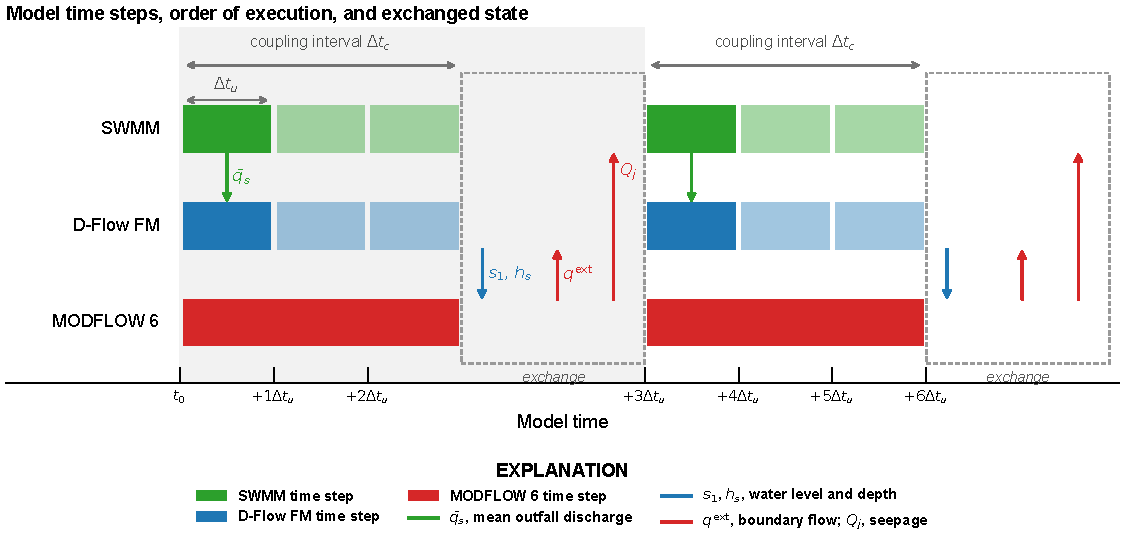
\includegraphics[width=\textwidth]{figures/coupling_sequence.pdf}
\caption{Model time steps, order of execution, and state exchanged among the three
simulators over two coupling intervals. Bar width is the model time step each
simulator integrates: MODFLOW~6 advances the whole coupling interval,
$\Delta t_c$, in one step, while SWMM and D-Flow FM tile that same span with one
bar per user time step, $\Delta t_u$. Lanes are ordered by execution rather than
by physical position. Every connector leaves the \emph{end} of the model time step
that produces a value and enters the \emph{start} of the model time step that
consumes it, so its horizontal run can be read against the time axis as the offset
between the two. Within a user time step SWMM advances first, so that its outfall
covers the interval D-Flow FM is about to integrate; the mean outfall discharge
over that step, $\bar{q}_s$, therefore returns one user time step to enter the
D-Flow FM step spanning the same interval. The second and third user time steps
repeat this and are drawn faded, with the exchange shown only once. At the end of
each coupling interval the D-Flow FM water level and water depth, $s_1$ and $h_s$,
are mapped to the MODFLOW~6 coastal boundary; that connector returns across the
whole interval, because the state read at its end is the boundary condition for
the MODFLOW~6 step spanning that same interval, which is consistent with the
backward-in-time step MODFLOW~6 takes internally and introduces no lag. The
boundary flow, $q^{\mathrm{ext}}$, and the aquifer--sewer seepage, $Q_j$, cannot
be recovered until MODFLOW~6 has finalized that step, so both run forward into the
interval about to start; that one-interval lag is the coupling error the sweep in
this study bounds. $Q_j$ is drawn in a neutral color and as a junction rather than
as a line between two models, because it belongs to neither: two thin arms collect
the end-of-step MODFLOW~6 head and SWMM water surface in the pipe, and two arms
deliver the resulting flux, equal and opposite, to the start of the next step in
each. One consequence is worth reading off the figure directly---a single
MODFLOW~6 step takes its coastal boundary at its \emph{end} and its sewer flux at
its \emph{start}. The exchange break occupies no model time---both of its edges carry the
same tick---and is drawn only wide enough to keep the two MODFLOW~6 blocks apart,
which would otherwise abut and read as one continuous step. A faded
stub at the right is the interval that follows, drawn so those connectors end on a
model time step rather than in blank space. Three user time steps per coupling
interval is the ratio at the finest interval simulated here; it reaches 288 at
daily coupling.}
\label{fig:sequence}
\end{figure}

The explicit scheme is imposed by what the interfaces expose, not chosen for
convenience. An implicit coupling requires every participant to re-evaluate a time
step against revised exchange terms, and only one of the three permits it: the
MODFLOW application programming interface exposes the nonlinear solution within a
time step, so the groundwater solution can be iterated
\citep{hughes2022modflowapi}. The hydrodynamic and sewer interfaces do not. Both
publish entry points that bracket a time step and advance it, with no facility to
re-solve the same step once an exchanged quantity has changed, so a coupled
iteration has nothing to iterate on two of its three legs.

The disparity in time step compounds the difficulty. The hydrodynamic model
advances on a user time step of seconds to minutes, the groundwater model on the
coupling interval, and the sewer model routes internally on a step of its own, so
the models step at rates differing by up to two orders of magnitude. Even were
re-evaluation available throughout, defining a converged coupled state across
those scales, and deciding which model repeats how many of its own steps per
outer iteration, is not a matter of simply looping the exchange. Quantifying how
the explicit solution depends on the exchange interval, which the demonstration
below does, is the useful thing that can be established without it.

The coupling interval is the principal numerical control on the approach. The
coastal boundary of the groundwater model is forced by a semidiurnal tide with a
period of approximately \SI{12.42}{\hour}, so a coupling interval that is a
substantial fraction of that period samples the tidal signal sparsely and
aliases it. Coupling intervals of 15 minutes, 30 minutes, and 1, 2, 4, 8, and 24
hours were simulated on each of three D-Flow FM grids to bound this effect.

\section*{Coastal exchange}

Water levels simulated by D-Flow FM are applied to the MODFLOW~6 coastal
boundary, which is represented by a General-Head Boundary (GHB) package covering
the inner bays and a Constant-Head (CHD) package covering the open coast and the
lateral perimeter. The D-Flow FM grid and the MODFLOW~6 grid are not
coincident, so the exchange is mediated by area-weighted mapping matrices
computed once, before simulation, from the intersection of the two grids.

The boundary head assigned to GHB cell $i$ is

\begin{equation}
  h_{i}^{\mathrm{GHB}} = \gamma \sum_{j} w_{ij}^{\mathrm{GHB}} \, s_{j} ,
  \label{eq:ghbhead}
\end{equation}

\noindent where $h_{i}^{\mathrm{GHB}}$ is the boundary head of cell $i$ (L),
$w_{ij}^{\mathrm{GHB}}$ is the area-weighted contribution of D-Flow FM cell $j$
to MODFLOW~6 cell $i$ (dimensionless), $s_{j}$ is the water level simulated by
D-Flow FM in cell $j$ (L), and $\gamma$ is the unit conversion from meters to
feet (dimensionless). Constant-head values are computed identically using the
corresponding CHD mapping.

Intertidal cells alternately wet and dry over a tidal cycle. A D-Flow FM cell
with zero water depth contributes no head and no conductance, so the GHB
conductance is reduced in proportion to the wetted fraction of the contributing
cells,

\begin{equation}
  C_{i}^{\mathrm{GHB}} = C_{i}^{0} \sum_{j} w_{ij}^{\mathrm{GHB}} \, \delta_{j} ,
  \label{eq:ghbcond}
\end{equation}

\noindent where $C_{i}^{\mathrm{GHB}}$ is the conductance applied to cell $i$
(L$^{2}$T$^{-1}$), $C_{i}^{0}$ is the conductance of cell $i$ in the base model
(L$^{2}$T$^{-1}$), and $\delta_{j}$ is unity where D-Flow FM cell $j$ is wet and
zero where it is dry (dimensionless). The base-model conductance, rather than
the conductance from the preceding coupling interval, is used on the right-hand
side of equation~\ref{eq:ghbcond}; applying the reduction multiplicatively to
the previous value would drive the conductance monotonically toward zero over
the simulation.

Boundary flows simulated by MODFLOW~6 are returned to D-Flow FM as an external
volume source. The source applied to D-Flow FM cell $j$ is

\begin{equation}
  q_{j}^{\mathrm{ext}} = -\beta \, \delta_{j}
    \left( \sum_{i} a_{ji}^{\mathrm{GHB}} Q_{i}^{\mathrm{GHB}}
         + \sum_{i} a_{ji}^{\mathrm{CHD}} Q_{i}^{\mathrm{CHD}} \right) ,
  \label{eq:qext}
\end{equation}

\noindent where $q_{j}^{\mathrm{ext}}$ is the volumetric source applied to
D-Flow FM cell $j$ (L$^{3}$T$^{-1}$), $a_{ji}$ is the area-weighted
contribution of MODFLOW~6 boundary $i$ to D-Flow FM cell $j$ (dimensionless),
$Q_{i}$ is the boundary flow simulated by MODFLOW~6 (L$^{3}$T$^{-1}$), and
$\beta$ is the unit conversion from cubic feet per day to cubic meters per
second (dimensionless). The sign convention of MODFLOW~6 reports boundary flow
as positive into the groundwater model, so the leading negative sign renders
$q_{j}^{\mathrm{ext}}$ positive into the surface water. Dry cells receive no
source.

\section*{Sewer exchange}

Exchange between the aquifer and the sewer is computed at a set of junctions
that fall within the active area of the groundwater model. Each junction is
associated with the MODFLOW~6 cell containing it, and a well is added to the
groundwater model at that cell.

Infiltration and exfiltration are driven by the difference between the
groundwater head and the water surface inside the pipe, and are limited by a
conductance representing the leakage area of the pipe wall served by the
junction. A per-junction conductance is computed from the sewer geometry as

\begin{equation}
  C_{j} = \lambda \, \pi D_{j} L_{j} ,
  \label{eq:pipecond}
\end{equation}

\noindent where $C_{j}$ is the leakage conductance of junction $j$
(L$^{2}$T$^{-1}$), $\lambda$ is a bulk pipe-wall leakance (T$^{-1}$), $D_{j}$
is the conduit diameter (L), and $L_{j}$ is the length of pipe served by
junction $j$ (L), taken as half the length of every conduit that the junction
touches. The served length varies by more than a factor of twenty across the
network, from approximately 28 to \SI{677}{\foot}, so a conductance assigned
uniformly per connection cannot represent the network geometry.

The driving head depends on whether the water table reaches the pipe. Where the
groundwater head stands above the pipe invert the surrounding material is
saturated and the gradient is measured to the water surface within the pipe;
where the head falls below the invert the pipe free-drains through unsaturated
material and the gradient is set by the depth of water in the pipe alone. The
driving head is therefore

\begin{equation}
  \Delta h_{j} =
  \begin{cases}
    h_{j} - \left( z_{j} + d_{j} \right), & h_{j} > z_{j} \\[4pt]
    -d_{j},                                & h_{j} \le z_{j}
  \end{cases}
  \label{eq:pot}
\end{equation}

\noindent where $\Delta h_{j}$ is the driving head at junction $j$ (L), $h_{j}$
is the simulated groundwater head in the cell containing junction $j$ (L),
$z_{j}$ is the pipe invert elevation (L), and $d_{j}$ is the depth of water in
the pipe above the invert (L). Positive $\Delta h_{j}$ produces infiltration
into the sewer and negative $\Delta h_{j}$ produces exfiltration. Treating the
disconnected case as $-d_{j}$ rather than $h_{j} - z_{j}$ is the same treatment
given a disconnected stream, and it is necessary: the latter form produces
exfiltration from an empty pipe that grows without bound as the water table
falls.

The exchange at junction $j$ is

\begin{equation}
  Q_{j} = \eta_{j} C_{j} \Delta h_{j} ,
  \label{eq:swmmq}
\end{equation}

\noindent where $Q_{j}$ is the exchange (L$^{3}$T$^{-1}$), and $\eta_{j}$ is
unity for infiltration and an exfiltration ratio less than unity for
exfiltration (dimensionless). Exfiltration into saturated material is more
difficult than infiltration from it, and the asymmetry is retained. The
exchange is applied to SWMM as a generated inflow at the junction and to
MODFLOW~6 as an equal and opposite well flux, so that mass is conserved between
the two models. Cells that are dry or inactive return a head of $-10^{30}$ in
MODFLOW~6 and are assigned zero exchange rather than being used unguarded.

\section*{Sewer discharge tracer transport}

Flow reaching the outfall is introduced to D-Flow FM as a point source carrying
a conservative tracer of sewer discharge, which is then advected and dispersed by the
hydrodynamic model. The source discharge is the total inflow simulated by SWMM
at the outfall, and the tracer concentration assigned to that discharge is
constant, so the tracer mass flux follows the simulated SWMM outfall discharge
directly.

The SWMM outfall discharge is written into the D-Flow FM source term at each
user time step. SWMM is advanced one user time step ahead of D-Flow FM so that
its outfall covers the interval D-Flow FM is about to integrate, and the
discharge applied over that interval is the mean

\begin{equation}
  \bar{q}_{s} = \frac{V\!\left(t + \Delta t_{u}\right) - V\!\left(t\right)}
                     {\Delta t_{u}} ,
  \label{eq:blockmean}
\end{equation}

\noindent where $\bar{q}_{s}$ is the mean SWMM outfall discharge over the user
time step (L$^{3}$T$^{-1}$), $V$ is the cumulative volume conveyed through the
SWMM outfall (L$^{3}$), and $\Delta t_{u}$ is the D-Flow FM user time step (T).
Forming the mean from the cumulative volume conserves mass exactly over the
step, whereas sampling the SWMM outfall discharge instantaneously once per
coupling interval and holding it would introduce the same aliasing that the
coupling interval itself is being tested for. Advancing SWMM at the user time step rather
than at the coupling interval does not alter the sewer solution, because SWMM
routes internally at its own routing step in either case and the exchange
computed from equation~\ref{eq:swmmq} is still refreshed only once per coupling
interval; it raises the resolution at which the outfall is observed.

\section*{Implementation}

The coupled simulation is implemented in Python. The three simulators are loaded
as shared libraries into a single process, so that state is passed between them
as arrays in memory.

D-Flow FM applies its external forcings at the start of a user time step and
then computes the flow solution. A source term written from outside the model
between those two operations is used by the solution, whereas one written around
the complete time step is overwritten by the forcing update before it is
reached. The direct tracer mechanism therefore advances D-Flow FM through the
separate initialization, computation, and finalization entry points of its
interface rather than through the combined update, and writes the source term
between the first and the second. This is the transfer drawn as $\bar{q}_s$ in
figure~\ref{fig:sequence}; the arrow falls within a user time step, not between
two of them.

This is the sub-time-step access described earlier, and the two simulators reach
it differently. MODFLOW~6 extends the Basic Model Interface with functions that
expose the time step and the solution within it \citep{hughes2022modflowapi}, and
those functions are what the groundwater exchange is written through. D-Flow FM
instead publishes its user time step as three separate entry points alongside the
combined one. Neither route is part of the Basic Model Interface itself, so a
coupling of this kind is portable only to the extent that each simulator provides
some equivalent.

\section*{Demonstration}

The coupling is exercised on the Greenport sewer network described above. The
groundwater model is a cutout of the regional Long Island aquifer system model
\citep{walter2024longisland}, which simulates the period 1900 to 2019 with
MODFLOW~6 including the position of the saltwater interface. Three D-Flow FM grids
of increasing resolution were used, spanning the same domain and driven by the
same tidal and atmospheric forcing. The groundwater and sewer
models are identical across all simulations, so differences among grids reflect
the resolution of the coastal water level alone, and differences among exchange
intervals reflect the coupling alone. The configurations simulated are
summarized in Table~\ref{tab:scenarios}.

\begin{table}[ht]
\centering
\caption{Simulated configurations. Each grid was simulated at every coupling
interval, giving 21 simulations in total.}
\label{tab:scenarios}
\begin{tabular}{lrrr}
\toprule
D-Flow FM grid & Cells & User time step (s) & Simulation period (d) \\
\midrule
Coarse  &  6,491 & 300 & 89 \\
Medium  & 16,666 & 300 & 89 \\
Fine    & 41,091 & 300 & 89 \\
\bottomrule
\end{tabular}
\end{table}

\section*{Results}

% Placeholder. Added here, with the supporting figures:
%   - sensitivity of the coupled solution to the exchange interval, which is the
%     numerical result the demonstration exists to produce
%   - whether that sensitivity is grid-independent
%   - what the exchange interval costs in run time, so the requirement can be
%     weighed against it
% Site-specific interpretation belongs only insofar as it bounds the coupling.

\section*{Summary and conclusions}

% Placeholder. Prose paragraphs, not bullets, once the analysis is complete:
% the coupling approach and what it costs; the character and bounds of the error
% introduced by the exchange interval, and how frequently the exchange must occur;
% and what the demonstration establishes about the requirements a library
% interface must meet for this kind of coupling -- that sub-time-step access is
% needed, that the Basic Model Interface does not define it, and that both
% simulators here supply it by different and non-portable routes.
%
% Forward-looking paragraphs close the section:
%   - what an implicit coupling would require that is not available today: the
%     hydrodynamic and sewer interfaces advance a time step but cannot re-solve
%     one, so two of the three legs have nothing to iterate on, and the models
%     step at rates differing by up to two orders of magnitude. This is a request
%     of the simulators, not a limitation of the approach.
%   - applying the same pattern to other simulator combinations, which requires
%     only that each expose an equivalent sub-time-step entry point

\section*{Acknowledgments}

% Placeholder.

\section*{Authors' Note}

The authors do not have any conflicts of interest to report.

\section*{Disclaimer}

Any use of trade, firm, or product names is for descriptive purposes only and
does not imply endorsement by the U.S. Government.

\bibliographystyle{elsarticle-harv}
\bibliography{gp_coupling}

\end{document}
